\chapter{Design and methodology}
This chapter presents the architecture of the system. Starting with a basic schematic view, it is showed what fundamental components compose it, their role, how they work and how they communicate each other.
%Then description of specific choiches
Then, the architecture is detailed more. Each step, starting with the download of raw activities and ending with the final user's attitudes, is described specifying what choices have been done and why.

At a high level, the system takes as input an ID representing a user in the system.
This user is associated with many IDs, one for each social network he or she is registered in and has provided access to.
These are used to download her profiles which, together with their respective activities, are used to classify the user's behavioural aspects included in the analysis.

\section{Requirements}
The main functional requirement is that the system has to be able to extract a set of behavioural aspect that characterise the user taken as input.
All the social network the user has registered must be analysed for both the social profile and the activities.
The architecture should allow the addition of new users into the system and the removal of existing ones. Then, once a system user is created, it must be possible to register and remove new social media account.
During the download of new activities, the system should let use a filter or a counter to exclude unnecessary activities.
Finally, the set of attitudes that can be classified must be defined a priori. For example, it can be equal, but not limited, to the 4 cognitive functions of the MBTI previously introduced.

\section{Process logic}
Here, the fundamental process followed by the system is introduced.
Each step covers a section of the process required to go from the simple user ID to the final insights that the system aims to provide.
The whole flow is sequential. Each activity takes as input the output of the previous one
There are 4 essential steps which can not be excluded despite specific design choices:
\begin{enumerate}
    \item Download profiles and activities from social networks.
    \item Analyse the downloaded data to extract significant features.
    \item Classify the profiles.
    \item Put together the partial results from each classifier to generate the complete user image.
\end{enumerate}
The steps are executed the same number of times and each one immediately follows the previous one with the requirement that the former must have ended for the latter to start.
The only exception can be found for the first two activities which could be grouped together. Indeed, once an activity is downloaded this could be immediately sent to the following action while a new one is put on download.
However, before the classification could be performed the whole profiles should be completely downloaded and analysed.
Finally, the final result can be stored. So, all the process is coordinated by a single call which start with the download phase and end the annotated user.

%This steps describe abstractally the flow followed by the system
%These functionalities are later in different components which purpose is to follow this process.
These steps give a general description of all the jobs required to go from the raw user identifier to its classification.
These functionalities are subsequently realized thanks to different components with the purpose of following this abstract process.
The final components of the system may vary according to the architectural choices made.

\section{Classificator's architecture}
While the first two steps are quite common and do not present significant choices that could modify the system, the third one deserve to be observed in more detail.
In the extraction of insights at user level, it is essential to understand precisely how the social user is defined and by what data it is characterised.
The state of the art rarely took into consideration different approaches. Usually, all the information obtainable by the totality of the activities downloaded are put together to represent the user ready to be classified.
It means that, at each request, all the downloaded activities are merged into a single user that summarise what has been provided by the social media.
At first, a solution of this type might work if the goal is to verify the feasibility of a specific classification in order to be able to measure its performance quickly and easily.
On the other hand, when it comes to the production environment, this technique presents some evident lacks that need to be considered.
For example, one main issue concerns the integration of the insight once new activities are posted by a user. %The integration of the result once new activities are posted. We don't want to recompute entirely the profile
The system should only download and classify the new activities and then integrate the result with the one previously stored.

Starting from this last problem I worked on three different alternatives. These three proposals are the feasible solutions that answered to a series of questions and critical points that emerged during this design process. 
\begin{itemize}
    \item Architecture \textbf{per aggregation}: the classification is performed on the so-called user aggregates. User aggregates represent the totality of the feature extracted by the profile and its activities. In the moment new activities are downloaded from the social profile, the previous aggregates are updated and then stored ready for the classifications.
    \item Architecture \textbf{per activities}: each activity is classified singularly. Instead of the features, the result of each activity is stored and then put together to generate the insight at a user-level.
    \item Architecture \textbf{per batch}: the classification is performed on the aggregates obtained from a batch of activities. Batches are disjoint sets of downloaded activities. Each is classified independently and its result is stored. These partial results of a specific user are merged together to get the final result. 
\end{itemize}

I evaluated and compared these three alternatives against six criteria considered fundamental with respect to the initial research question.
The six bases are: computation complexity, result's accuracy, GDPR compliance, result's flexibility, storing, and scalability.

\subsection{Computation Complexity}
The performance of each propose strictly depends on the trade-off between a single classification and the aggregation of features from many activities.
Assume that the cost of a single classification is equal to the number of features M, $\Theta(M)$.
Estimate now, for each solution, the computational complexity of the download of N activities and the user's classification.
Firstly, It must be noticed that the first two steps of the process, the activities download and their analysis, are not affected by the architectural choice. Therefore, to keep everything clearer, their contribution will be omitted from the following estimations.

Assuming that the aggregation algorithm just iterate on each post of the timeline a single time observing each one of the M extracted features. So, its computational cost is $\Theta(N*M)$.
As already said, Using user's aggregates implies to compute the classification on its totality at every request to the system. So, this method's complexity considers the number R of requests which is obviously constantly growing. 
It can be formalized as \textbf{$\Theta(N*M) + \Theta(M*R)$}.

Regarding the second alternative, while it is no longer necessary to aggregate the analysis of each activity, it is required to merge together each singular result in order to obtain the final insight.
Moreover, the classification is performed N times on the exact number M of features.
So, the complexity of the solution activity-based is \textbf{$\Theta(N*M) + \Theta(N)$}.

To analyse the last solution, the batch-based one, it is not necessary to define how batches are composed in detail.
The N downloaded activities are somehow partitioned into B batches with $B \leq N$.
Each batch's content is aggregated with the same algorithm introduced before. In general, it is not important how many batches there are, the aggregator will still work on M features of the N activities.
Finally, the B batches are classified singularly and their results are then joined together.
So, the complexity is \textbf{$\Theta(N*M) + \Theta(B*M) + \Theta(B)$}.

To conclude, since the architecture aggregation-based considers in its formula the number of requests to the system, it is not scalable in terms of increasing loads.
On the other hand, the other two alternatives are computationally similar. The differences between the two stay in the number of classifications done and the final aggregation of partial results.

\subsection{Accuracy of the result}
Regarding the final result obtained by each of these three methods, even though it would be better to carry out a detailed evaluation process, some general observations can be done without any implementation test.

Starting with the architecture per batch, user aggregates are easy to calculate since they generally consist in the sum of many values or in their average. Thus, they are precise and represent correctly the user's values.
However, even though until now I have been talked only about features extracted by the online activities of the user, other useful information is represented by that related to the social profile. For example, fields such as the number of followers, that of people followed, the user's location, and many other help describing the individual, her social presence and connections.
In this case, at every download request, this information contained in the user aggregate is updated with the new one. Consequently, the snapshot of the old status is lost.
This means that the activities are not associated with the exact moment they were written but they all treated the same way without differentiating the social situation of the user.

This last issue is partially solved by the activity-based methodology because in the features used to classify each activity can be included that information about the social user.
However, this data is taken in the moment the social network's API are consulted so it is not perfectly accurate for each post but it can represent a good approximation.
On the other hand, this alternative involves two major obstacles. Firstly, it has been proved that, especially in the case of psychological studies, text represent the first source of information. Typically, on the social media, users tend to write short posts composed by just a pair of sentences. 
Thus, what has been argued is that the quantity and the quality of the extracted features do not allow a precise classification of behavioural aspects.
Secondly, once every single activity is classified, they must be merged together to generate the user's insight.
In the case of categorical results it is not clear how singular results should be merged and how each one should be weighted with respect to the others.

Finally, the architecture per batch has the same advantage of the one per activities because each batch would be characterised by the features that describe the social status of the user.
So, each batch of activities, depending on when its was downloaded, includes some data describing that information mentioned before.
Moreover, the problems of the previous technique here are less pronounced. Indeed, batches can include the right number of activities in order to get the right amount of features.
Also, during the aggregation of partial results, each one could be weighted both dimensionally and temporally giving so more freedom to adapt the implementation.


\subsection{GDPR Compliance}
Design a system that respect the last regulations about the protection of personal data is one of the goals of this thesis.
In this design phase, some requisites from the GDPR emerged as crucial aspects. In this chapter it is explained how the three different architectures satisfy or not the requisite of data minimisation and that of data accuracy already introduces in chapter 2 "State of the Art".

Starting as always from the solution per aggregation, it implies to store the user aggregates so that they can be updated or classified whenever the user wants.
Even though this data is composed by the relative features extracted from the activities and not by the activities themselves, they still contain personal and sensitive that need to be protected.
Then, as discussed is the previous section, info about the social status are unique and dated to the last upload so they are less accurate with respect to the whole timeline.

Using one of the other two alternatives, the situation changes markedly because they do not require to store the activities nor the extracted features. It is enough to memorise all the partial results and some descriptive information, such as the number of activities and their date, in order to be able to join them together.
The solution activities-based, compared to the last one, brings more profit with respect to the accuracy issue. Indeed, it gives the opportunity to complement every single activity with the social status in the moment it was posted while batches still implies a minimum approximation.

\subsection{Flexibility of the result}
This small chapter gives a focus on the benefits regarding the result's flexibility rather than criteria that need to be met.
Depending on this architectural choice the system could allow the composition of the final results with different options. For example, by taking into consideration only a subset of the whole user's timeline

Using the user aggregates, it is quite difficult to act on the final result once it has been classified.
Indeed, the result is the direct output of the subset of aggregates the classification algorithm uses. So, the only way to affect the result is by working on these aggregates which include the whole timeline and are unique for each user.
%Quindi l'unico modo per "filtrare" l'input del clasificatore sarebbe quello di riscaricare ed analizzare nuovamente solo le attività che rispettano il filtro desiderato

The architecture activities-based is for sure the one with the highest flexibility. Indeed, it is immediate excluding some activities that do not meet a specific requirement.
For example, it would be possible to compute the user only for her social presence during the summer periods or during the weekends. 
So, memorising a flag together with the result would be enough to subsequently filter the final result.
These flags are not limited only to datetime aspects. For instance, they can be used to differentiate posts that talk about sports from those that talk about politics.

With the solution based on batches, it becomes possible to treat each batch differently. It all depends on how the batches are composed.
For example, batches that cover specific time periods give the opportunity to observe temporal variations. Then, they could be filtered depending on a exact term.
Also, each batch can be normalized regarding the number of activities it contains in order to weigh its contribute on the final result.


\subsection{Storing}
Here is briefly discussed where, in the system, data persistence needs to be implemented
Then, it is observed how the data model affects the system and, in particular, its evolution.

To compute the user aggregates, persistence must be implemented on the component that perform the aggregation so that they can be updated at every new download.
Then, the results of the classifications need to be stored. Also, the activities collector should know which is the last activity downloaded for each user in order to not count them multiple times.
The features the system memorise are always known a priori depending on what classifications the system performs. Consequently, the removal or the addition of some features, for example to improve or add a new model, involve adapting the whole data model and the download of the whole user's timeline.

For the other two proposals, it is necessary to have data persistence on the component that deals with the classifications so that the result of each batch or activities can be stored.
Obviously, the activities collector always need to know which is the last downloaded post.
It is quite immediate to add new services at the system since the features extracted do not need to be memorised but are immediately used from the next component. So, the data model is affected only on the result aspect in the case new classifications are added.

\subsection{Scalability}
This last aspect does not vary much from one solution to another. All three architectures allow the parallelization of the independent classifiers.
In addition, for the two architectures based on multiple classifications, these can be parallelized since both each batch and each activity are independent of the others.

%Capitolo nuovo

\section{Components's logic and interaction}
After this analysis, it was decided to focus on the third proposal, the batch-based architecture.
The one based on the user aggregates is quite basic has several shortcomings in many of the observed aspects.
The other two share many advantages but regarding the accuracy of the result, the activity-based solution has some complications not included on the other one.
However, as said before, that aspect was analysed through general observations and testing both the architecture would give a more detailed overview.

\begin{figure}[htp]
    \centering
    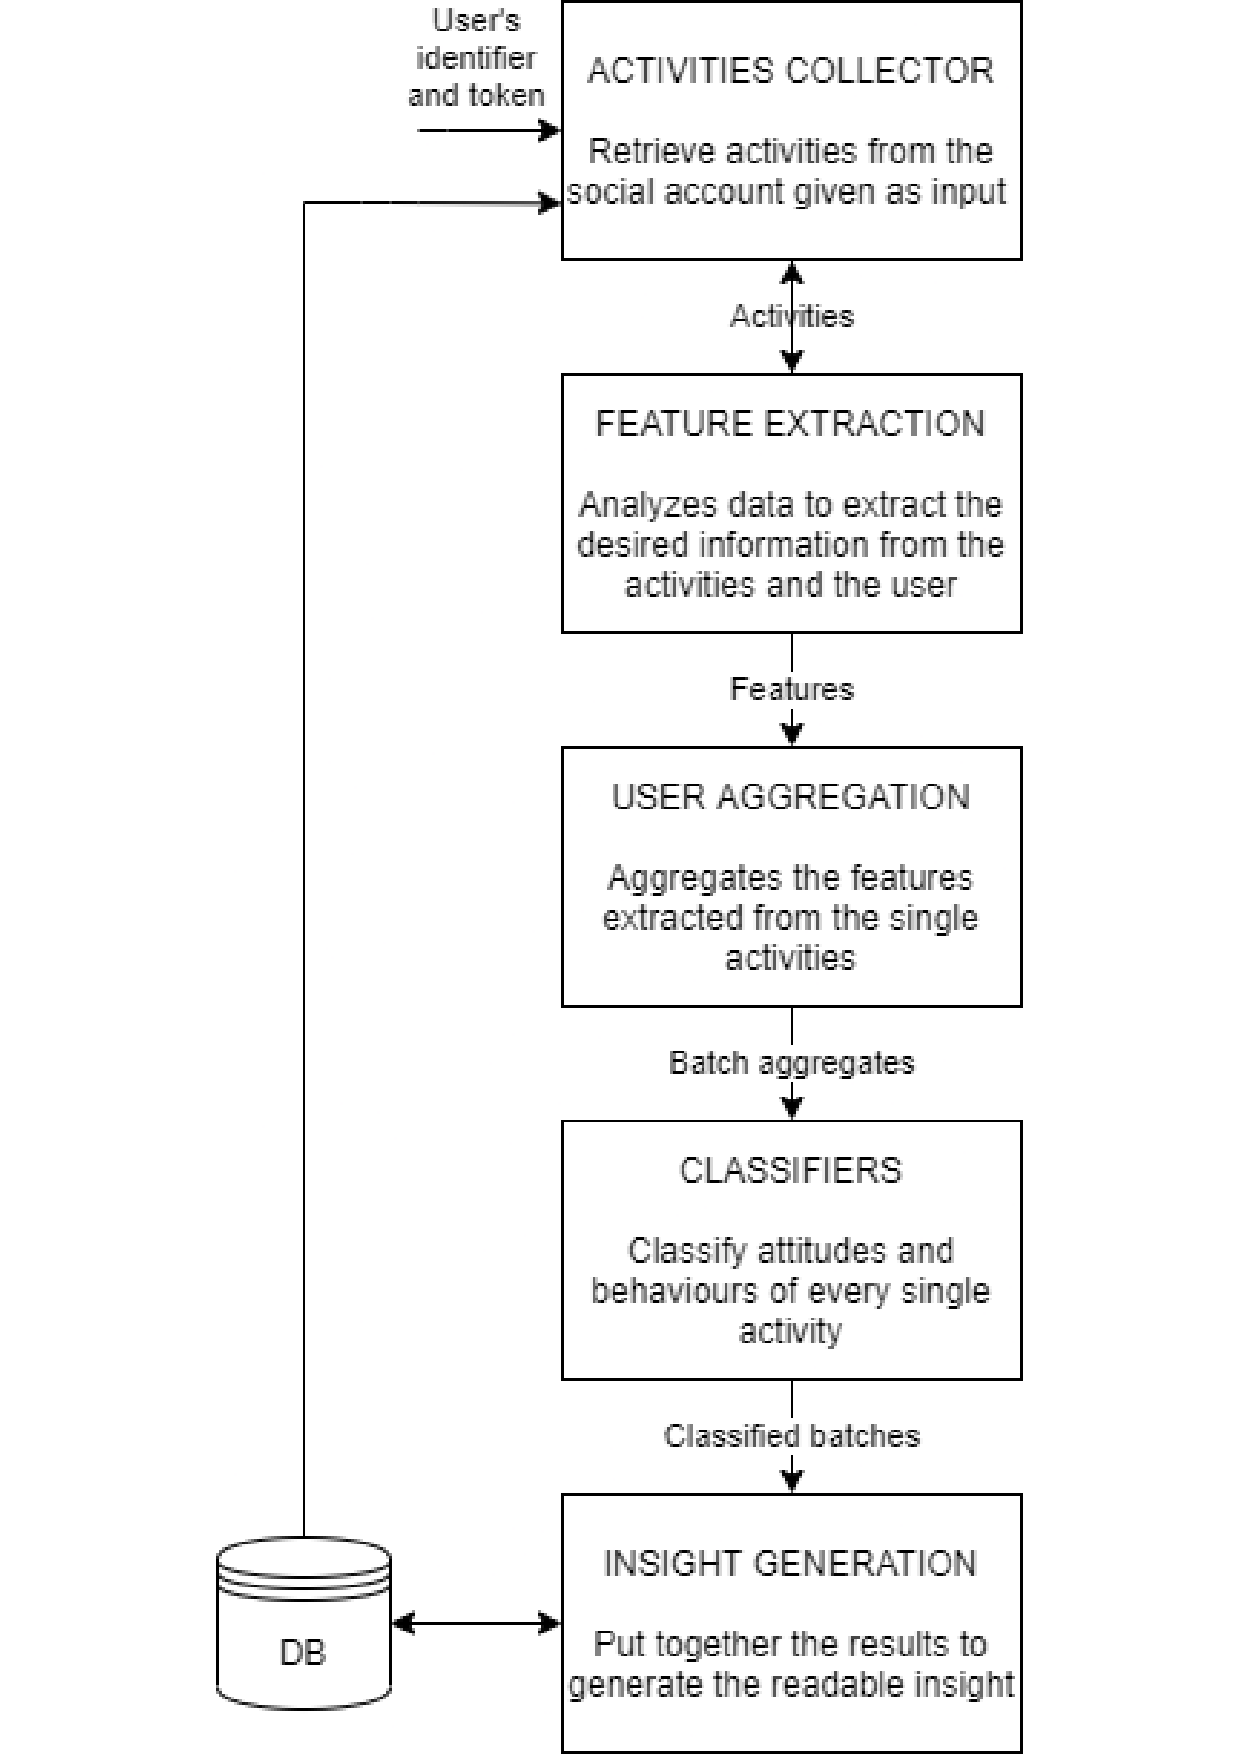
\includegraphics[width=%
    0.95\textwidth,height=10cm,keepaspectratio]{img/components}
    \caption{The architecture components}
    \label{fig:components}
\end{figure}

In this section, the architecture is decomposed into its components. Each component works on the input of the previous one to carry out a step of the whole process described previously.
Totally, 5 components have been identified: activities collector, features extractor, user aggregator, classifiers and the insight generator. They are shown in Figure~\ref{fig:components}:


Next, the logic of each component is provided, illustrating what each one does, its input, and output.
For each component, it is also presented its API. Internal APIs are used by the components to facilitate and standardise their interaction.
These components are presented as web interfaces that takes as input and returns as output JSON objects.
Only the parameters used to identify the object itself are used. For example, a postID and a socialID are enough to indicate an activity.

\subsection{Activities collector}
This part deals with the downloaded of user's content from social networks through the services offered by the public APIs of each platform.
The data includes information about the user, such as social name, number of followers and friends, location, and then her activities.
An activity is usually characterised by some text, optional attachments such as media or files, a creation date, the number of likes, shares and comments, and, sometimes, information derived from the geolocation.

This component takes as input a list of IDs, one for each social network connected to the user, that identify all her profiles. Some social media, like Facebook and Instagram, also require an access token necessary, together with the user ID, to consult, through the API, the content of that profile.
These tokens are released directly at the organization that is handling the user authorization.

For each social network, the system need to know at which point the data has been previously downloaded. Usually, the IDs identifying the posts are ordered and the API allows you to specify the point the download should start from using an ID.
As output, the components returns a social profile composed by significant user's information and the list of new activities. With new, it is meant all the content that was not previously downloaded by past requests.
Finally, the last activity of the timeline is used to update the point the data has been fetched.

The collector interacts with many different social networks. To do it, this service should run in a dedicated process and the communications with each platform should be parallelized.
This is necessary because many socials provide free API plans which limit the number of requests in a given time window. So, in case one of the limits is reached, it should not cause a critical bottleneck that freezes the whole system.

\begin{multicols}{2}
\begin{verbatim}
//input
[
    {
        "socialID": 1234,
        "userID": 8564
    }
]

//output
[
    {
        "postID": 123456,
        "socialID": 1234
    }
]
\end{verbatim}
\end{multicols}

\subsection{features extractor}
This component works on the downloaded content to extract significant features for the following step.
From the previous part it receives data both about the user's information and about her activities. While the first one is quite structured and does not need deep analyses, the activities carry raw texts and images which have to be processed to extract the desired information.

First of all, the text of each activity is observed and analysed to extract significant features for the classification models, in particular for the psychological ones.
A standard \emph{Natural Language Processing NPL} library is used. It allows to observe some superficial characteristics such as the number of sentences, words, characters, capital letters and the use of punctuation.
Then, giving the environment we are working with, that of social media, it is important to handle properly hashtags, external links and emojis.

The first two, as well as any mention or @tag, are usually returned by the social network's API. So, it is not necessary to extract them from the raw text.
On the other hand, emojis are treated like any other character by the API. Therefore, they need to be parsed carefully.
Taking care of emojis is extremely important because on social media they are abused by the majority of users and, thanks to their variety and intuitiveness, they can reveal a lot about the traits of a person.

Another significant step of the natural language process is the \emph{Part-of-speech (POS)} tagging. It consists in assigning a particular part of speech,, such as nouns, verbs, and adjectives, to a specific word in the corpus.
Doing that, it is possible to observe, for example, how much a person tends to detail her messages by using adjectives or whether someone writes in the first or third person.

Then, we want to understand what the user has talked and posted about. Both text and images can be used to accomplish this goal; thanks to some external semantic analysers that can extract entities, topics, and a sentiment value.
These services usually use the Wikipedia tree to map both entities and topics. The first set refers to every concept that has its own page on Wikipedia. Differently, a topic is a Wikipedia category.
In the Wikipedia structure, each page can be characterised by many different categories. 
The sentiment is returned as a label that can be \textit{negative, neutral, or positive} or as an integer ranging between two values. For example, between -1 and 1 where -1 means extremely negative and 1 extremely positive.

At the end, this component returns as output the same user taken as input where each of her activities has been analysed. So, each post is replaced by the list of features extracted from it.
Every activity obviously has the same general feature names. In some cases, for example, if a text did not contain any Wikipedia entities, some may be empty but they are still contained in the returned object.

The feature extraction is not limited to the analyses mentioned here. The idea is that this component should be integrable with new services and functions.

\begin{multicols}{2}
\begin{verbatim}
//input
[
    {
        "postID": 123456,
        "socialID": 1234
    }
]
    
//output
[
    {
        "postID": 123456,
        "socialID": 1234
    }
]
\end{verbatim}
\end{multicols}

\subsection{Aggregator}
This part has to task to create a single object, characterised by a series of features, that is ready for the following classifications. It receives as input the social profile and its analysed activities.
By simply iterating over all the activities received, it is primarily responsible for dividing them in batches and then calculating their aggregated values.

The way batches are composed can not be decided a priori. Two different techniques for their composition have been identified.
A first one that works on a fixed number of activities for each batch and an alternative which divides posts into batches covering fixed time periods.

The dimensionality-based one is the most basic. Simply, if 180 new activities are downloaded and it is decided to compose batches of 50 activities each, three full and one-half batches will be returned.
This methodology is in contrast with the result's flexibility criteria seen above because any type of control over the individual activities is lost.

On the other hand, the temporality-based alternative divides batches in a more organized way.
In fact, there is an additional degree of freedom that allows you to decide the length of the time periods. 
This solution helps visualizing the result and giving the opportunity of observe how significant insights varies over time.
However, this period must be common for every set. In Chapter~\ref{cha:evaluation} a prototype of the system is implemented with batches covering one month.

After the various activities are divided, it is necessary to run the same aggregation algorithm on every batch.
At first, static information about the user's profiles, such as creation date and the number of friends are copied in each batch.
Then, for each set of features, the significant features are aggregated in the best way to represent them globally
So, for example, it is counted how many activities of each type there are. These can be differentiated into original posts, shares, comments and replies.
Then, text features are summed together treating the batch as a single text document.

Finally, a list of batches is returned. Each one includes all the data needed for the classifications implemented by the system.
Each batch should also contain some descriptive information such as the ID of the oldest activity it contains, the number of activities, and the time period that it covers.

\begin{multicols}{2}
\begin{verbatim}
//input
[
    {
        "postID": 123456,
        "socialID": 1234
    }
]
        
//output
[
    {
        "UserID": 8564,
        "batchID": 001
    }
]
\end{verbatim}
\end{multicols}


\subsection{Classifiers}
At this point the situation is that each batch represent a partial user who can be classified. 
This component has the goal to assign a value for each aspect implemented by the system.

This decision can be made both with machine learning and non-machine learning algorithms. Section~\ref{sec:Classifiers} gives a more detailed description of the classifiers included in the system.
In this thesis, as discussed later in Chapter~\ref{cha:evaluation}, machine learning models have been used for psychological aspects while better-defined characteristics, such as the users' activity periods over the day, are inferred by looking singularly at the features.

As showed in Figure~\ref{fig:components} all the classifiers are treated as a single component. Actually, there are many different classifiers.
Some may work on the same features but, in general, they are all independent from each other.
So, their execution can be viewed in parallel where, as it is shown in Figure~\ref{fig:classifiers} all the subcomponents use the same input and each one contributes to the generation of the final output

\begin{figure}[htp]
    \centering
    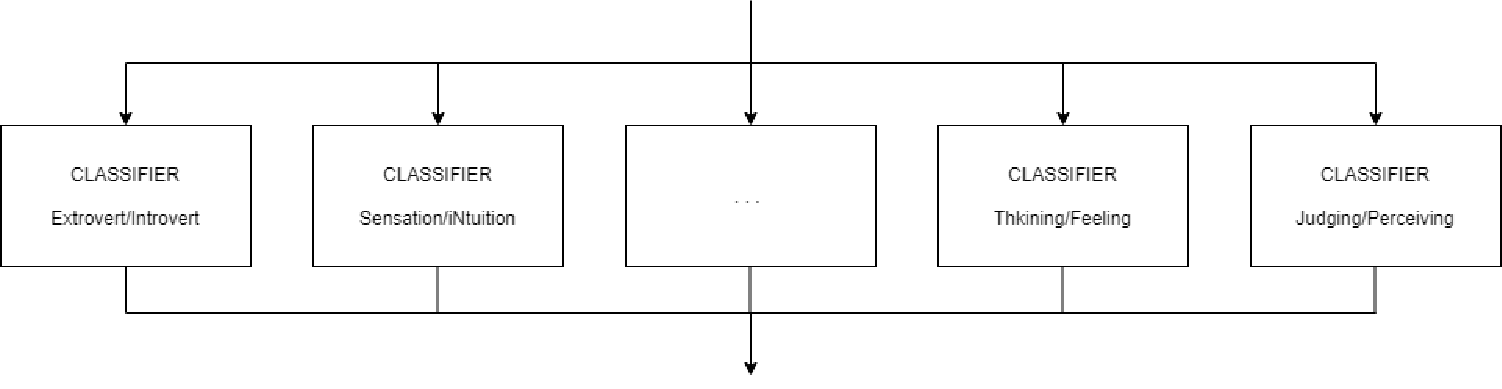
\includegraphics[width=%
    1.0\textwidth,keepaspectratio]{img/classifiers}
    \caption{Parallel view of some of the classifiers}
    \label{fig:classifiers}
\end{figure}

In the case of classifiers that use text features, it must be remembered that all the analyses done on natural language depend strictly on the language on the same.
Therefore, to handle multiple languages, multiple classifiers are required.

As output, the same list of input batches is returned where for each implemented aspect the corresponding class is returned.
%The result of each batch, together with its descriptive information, can now be stored.

\begin{multicols}{2}
\begin{verbatim}
//input
[
    {
        "UserID": 8564,
        "batchID": 001
    }
]
            
//output
[
    {
        "UserID": 8564,
        "batchID": 001
    }
]
\end{verbatim}
\end{multicols}

\subsection{Insight generator}
\label{sec:Generator}
DESCRIPTION OF THE ALGORITHM USED TO MERGE TOGETHER BATCHES' RESULTS

\section{Classifiers}
\label{sec:Classifiers}

In this section, each classifier supported by the system is described. There are both binary models, where the output is either 0 or 1, and multi-class classifiers that classify instances into one of N classes, with $N>2$.So, here the output ranges from 0 to $N-1$ and each integer represents a class.
In this way, all the models share a common structure for the representation of their results. The mapping from the integer to the descriptive category is carried out later when the user's result is requested.

A big issue in dealing with user profiling from social media is the lack of data. Indeed, even though many different aspects of a person have been studied, only a limited number of papers published the datasets they used or built for that research.
Since not enough data to train and evaluate a machine learning model is available, artificial intelligence solutions are not always viable.
For this reason, as introduced before, many of the algorithms presented here do not follow a machine learning approach but a more standard one.

\subsection{MBTI Personality traits}

\subsection{Daily Usage}

\subsection{Influence Role}

\subsection{Language}


\section{Exposed APIs}
Finally, the endpoint offered at the user by the system are presented. During the design of the interfaces, the principles of the RESTful architecture have been followed.
The resources publicly exposed are two: \textbf{User} and \textbf{New Activities Download}.
Regarding the user, it is possible to create new instances, modify, or delete existing ones.
A user is basically a list of social profiles and a name to be identified. Each social profile requires a user id and an access token.
When a new user is added to the system, it results as non-classified. The \textbf{New Activities Download} allows you download and classify her social profiles.
At this point, retrieving the user instance it will be classified and the extracted insights about her will be returned.
The complete API specification can be found on Apiary:

\begin{center}
\url{/uhopperthesis.docs.apiary.io}
\end{center}
